\headerbox{1. Abstract}{name=abstract,column=0,row=0,span=3}{
\vspace*{-2.0em}

\noindent\makebox[\linewidth][c]{%
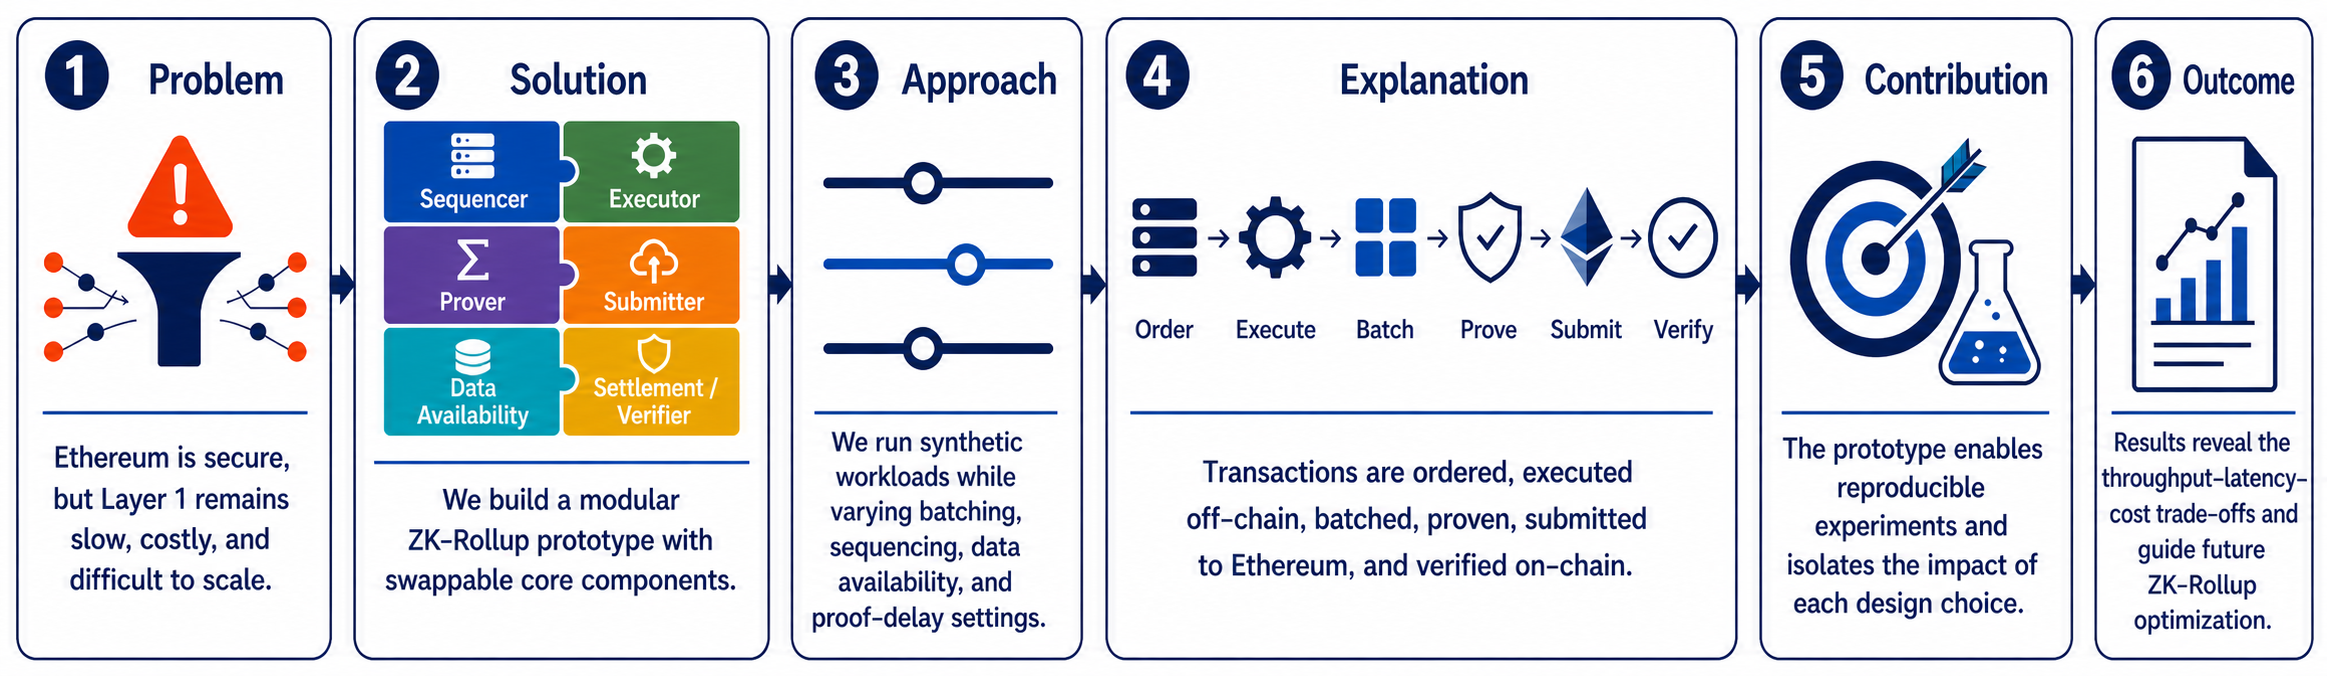
\includegraphics[
    width=1.06\linewidth,
    keepaspectratio
]{poster/images/abstarct.png}%
}

\vspace*{-2.0em}
}

% \headerbox{1. Abstract}{name=abstract,column=0,row=0,span=3}{

% \vspace{-0.4em}

% \begin{minipage}[t]{0.66\linewidth}
% \vspace{0pt}
% \normalsize
% \begin{itemize}[leftmargin=0.75em,itemsep=0.02em,topsep=0pt,parsep=0pt,partopsep=0pt]
%     \item \textbf{Problem:} Ethereum L1 has low throughput, high fees, and delayed finality.
%     \item \textbf{Solution:} ZK-Rollups execute transactions off-chain, batch them, and submit validity proofs to L1.
%     \item \textbf{Approach:} We implement a modular Rust-based ZK-Rollup with sequencer, executor, prover, submitter, and DA modules.
%     \item \textbf{Evaluation:} We benchmark batch size, sequencing policy, workload mix, and DA mode using TPS, latency, gas/tx, and proof time.
%     \item \textbf{Contribution:} A reproducible framework for studying ZK-Rollup throughput--latency--cost trade-offs.
% \end{itemize}
% \end{minipage}
% \hspace{0.01\linewidth}
% \begin{minipage}[t]{0.32\linewidth}
% \vspace{-1.0em}
% \centering
% 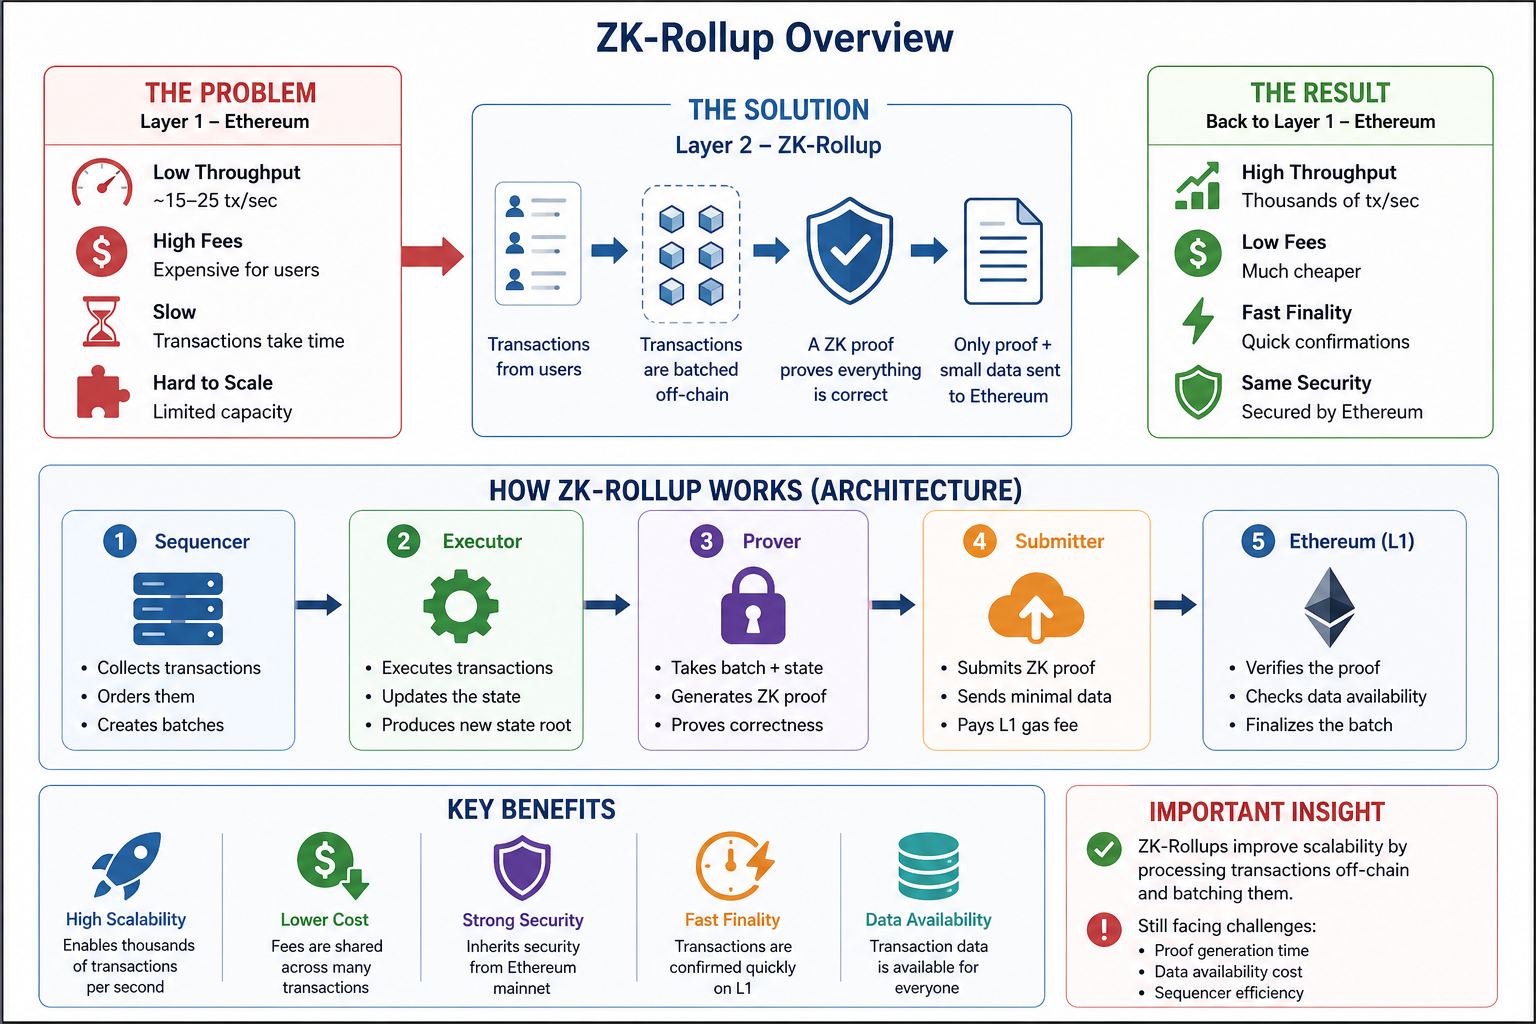
\includegraphics[width=0.92\linewidth]{poster/images/overview2.png}

% \vspace{-0.4em}
% {\scriptsize\textbf{Figure:} ZK-Rollup overview.}
% \end{minipage}

% \vspace{-0.8em}

% }